\chapter{Realisierung des IIR-Filters}\label{Cha:RealIIR}
\section{Aufgabenstellung}
Die Aufgabe dieser Übung bestand darin, einen IIR Filter zu realisieren. Dabei galt besonderes Augenmerk der Minimierung von Rundungsfehlern sowie der Verhinderung von Überläufen.
\section{Durchf\"uhrung}
Das Filter wird auf die nachfolgenden vier Varianten implementiert. Vorab wurden dazu die Filterkoeffizienten entsprechend der Aufgabe nach aufsteigendem Radius im Einheitskreis sortiert.

Es wurden wie in der Aufgabe beschrieben die Dateien in ein neues Projekt eingefügt und wie im folgenden beschrieben entsprechend angepasst.
\subsection{Skalierung am Eingang}
Die einfachste Form der Skalierung ist die Skalierung am Eingang, wobei mit einem Divisor vor verwenden des Filters dividiert wird. Dazu wird zuerst die gesamte Verstärkung der Filter durch Multiplikation ermittelt.
Da es sich um einen Tiefpass handelt wird die Verstärkung bei 0Hz berechnet. Es folgt: z=1.
Gemäß folgender Formel ergibt sich eine Gesamtverstärkung von 474.5917.
\begin{equation}
\Pi H_i(1)=38,3655*4,8221*1,8921*1,3558=474.5917
\end{equation}
Daraus folgt die Anpassung der Datei process\textunderscore data.c wie folgt.\\

\begin{adjustbox}{width=\textwidth,height=\textheight,keepaspectratio}
 \begin{lstlisting}[title=processdata.c]{processdata.c}
// Definition der Filterkoeffizienten
#define BIQUAD_STAGES 4

// coef includes for all stages a scaling factor (2^s) and five coefficients
// in the order s, b2, b1, b0, a2, a1

// No scaling in stages (Low Pass)
const short coef[6*BIQUAD_STAGES] = {
	1, 16384, 6581	, 16384, -10390, 25748  //H4
	1, 16384, -20909, 16384, -12529, 26454, //H3
	1, 16384, -25583, 16384, -14605, 27191, //H2
	1, 16384, -26706, 16384, -15896, 27808, //H1
};

int iDelayline[2*BIQUAD_STAGES+2];	// delayline for left and right channel samples

IIRstateStereo iirLR={coef,iDelayline,BIQUAD_STAGES};

void process_data()
{
	//!! Scale before filtering
	sADC1L = sADC1L / 474.5917; //skalierungsfaktor aus Rechnung
	sADC1R = sADC1R / 474.5917;
	*(int*)(&sDAC1L) = iir_stereo(*(int*)(&sADC1L),&iirLR);

	//!! Scale after filtering
}

\end{lstlisting}
\end{adjustbox}
Die Interpretierung als 1.15 Format findet sich in den eingetragenen Koeffizienten nicht, sie wurden als short implementiert. Die Konvertierung erfolgte wie in früheren Laborübungen gesehen. Die Implementierung als short ermöglicht eine bessere Übersichtlichkeit und vermeidet Fehler. Die Zweite Anpassung war die eigentliche Skalierung am Eingang, hierzu wurde der zuvor ermittelte Divisor verwendet.\\
\begin{figure}[H]
  \centering
    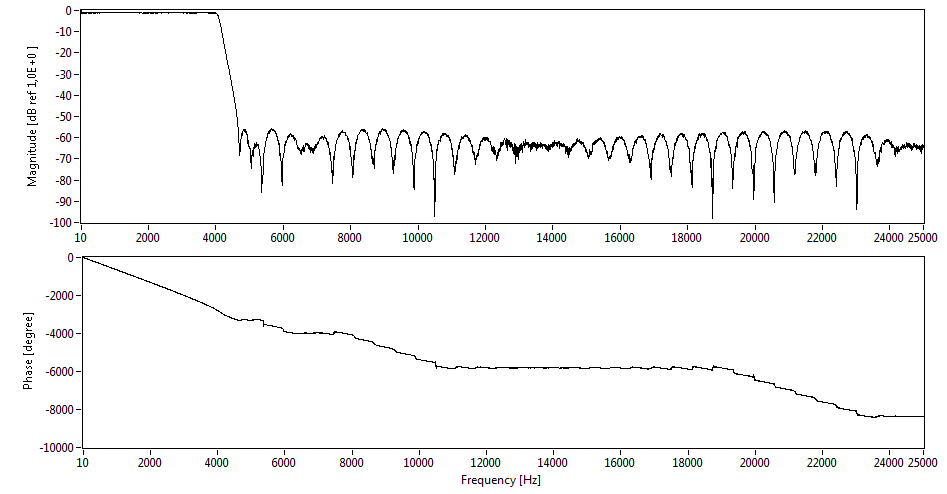
\includegraphics[width=\textwidth]{Freqgang3_1.png}
  \caption{Frequenzgang}
  \label{fig:Freqgang3_1}
\end{figure}
Hier wurde der Frequenzgang des Systems visualisiert, es ist deutlich das Tiefpassverhalten auszumachen. Die Grenzfrequenz liegt bei etwa 4kHz.\\
Zur weiteren Untersuchung wurde folgendes Sinussignal mit 2kHz Frequenz und 50mV Amplitude eingespeist.
\begin{figure}[H]
  \centering
    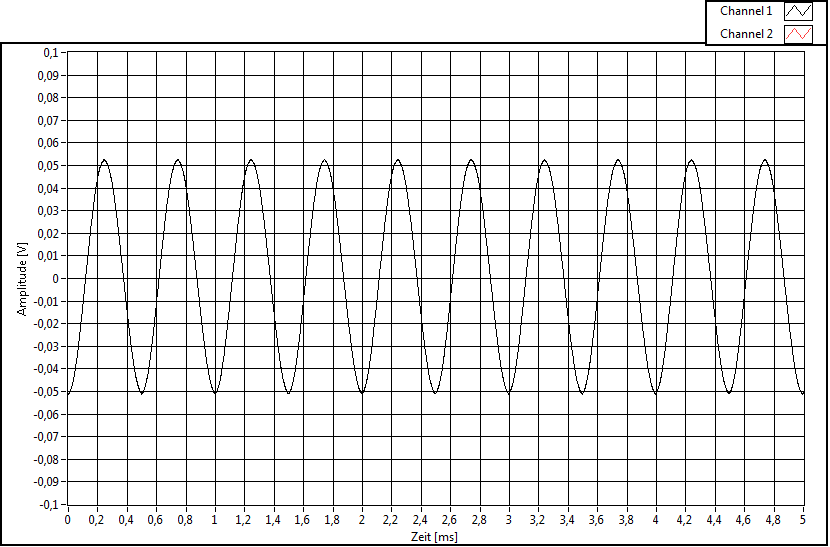
\includegraphics[width=\textwidth]{Eingangssignal50mv2kHz.png}
  \caption{Eingangssignal}
  \label{fig:Eingangssignal50mv2kHz}
\end{figure}
Wir haben am Eingang das nachfolgende Spektrum gemessen.
\begin{figure}[H]
  \centering
    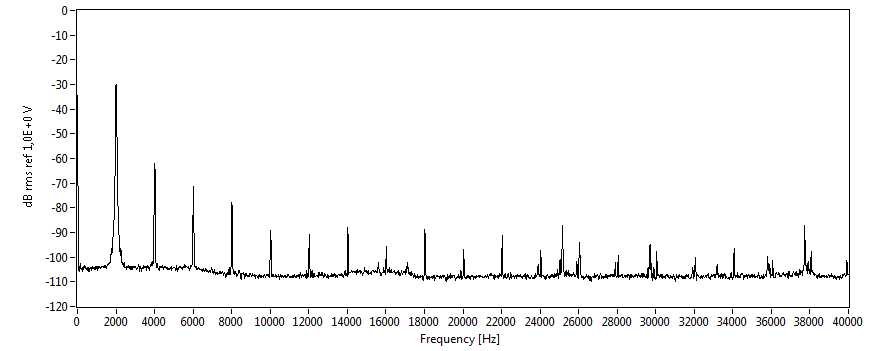
\includegraphics[width=\textwidth]{PowerspekEingang.png}
  \caption{Spektrum am Eingang}
  \label{fig:PowerspekEingang}
\end{figure}
Und am Ausgang hat man in nachstehendem Spektrum das Rauschen gut beobachten können.
\begin{figure}[H]
  \centering
    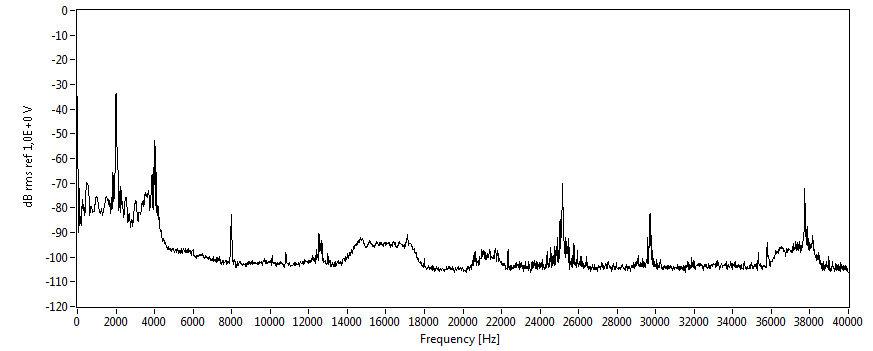
\includegraphics[width=\textwidth]{PowerspekAusgang.png}
  \caption{Spektrum am Ausgang}
  \label{fig:PowerspekAusgang}
\end{figure}
Es ist gut zu sehen, dass am Eingang mehrere Harmonische alle 2kHz zu sehen sind, umgeben von einem sehr geringen Rauschteppich bei unter -100dB. Am Ausgang hingegen ist das Tiefpassverhalten zu erkennen, was die erste Harmonische bei 4kHz (der Grenzfrequenz) noch leicht gedämpft darstellt, alle weiteren Harmonischen aber hinreichend unterdrückt. Außerdem lässt sich ein Rauschen ausmachen, was bis zur Grenzfrequenz um -80dB liegt. Dieses Bild entspricht unseren Erwartungen.
\subsection{Skalierung am Ausgang}
Entsprechend der Aufgabenstellung haben wir auch die Skalierung am Ausgang umgesetzt, wie erwartet übersteuerte das System massiv, was die Analyse der Implementierungsvariante unnütz machte. Aus diesem Grund verzichten wir wie Abgesprochen auf eine Auswertung an dieser Stelle.
\subsection{Gleichmäßige Skalierung}
Im dritten Teil der Übung wurde das Filter gleichmäßig über alle Teilfilter skaliert. Dazu wurde die Gesamtverstärkung aus dem ersten Teil gleichmäßig auf die Teilfilter aufgeteilt. Der Divisor ergibt sich also wie folgt:\\
\begin{equation}
\sqrt[4]{474.5917}=4,6675
\end{equation}
Bereits in der Vorbereitung wurden die Filterkoeffizienten durch diesen Quotienten geteilt und in das short Format gebracht. Somit ergibt sich folgende Änderung:\\
\begin{adjustbox}{width=\textwidth,height=\textheight,keepaspectratio}
 \begin{lstlisting}[title=processdata.c]
 
 // No scaling in stages (Low Pass)
const short coef[6*BIQUAD_STAGES] = {
	1, 3514, 1412, 3514, -2229, 5523, //H4
	1, 3514, -4485, 3514, -2687, 5674,//H3
	1, 3514, -5488, 3514, -3133, 5832,//H2
	1, 3514, -5728, 3514, -3410, 5965 //H1
};



int iDelayline[2*BIQUAD_STAGES+2];	// delayline for left and right channel samples

IIRstateStereo iirLR={coef,iDelayline,BIQUAD_STAGES};

void process_data()
{
	//!! Scale before filtering
	*(int*)(&sDAC1L) = iir_stereo(*(int*)(&sADC1L),&iirLR);
	//!! Scale after filtering

}

\end{lstlisting}
\end{adjustbox}
Es ist auch ersichtlich, dass die Skalierung am Ende im Gegensatz zur vorherigen Aufgabe entfernt wurde.\\
Bei dieser Art der Implementierung erwarten wir ab einer gewissen Amplitude Übersteuerungsfehler. So haben wir ein 2kHz Signal angelegt und die Amplitude sukzessiv erh\"oht und sind zu folgenden drei Bildern gelangt.
\begin{figure}[H]
  \centering
    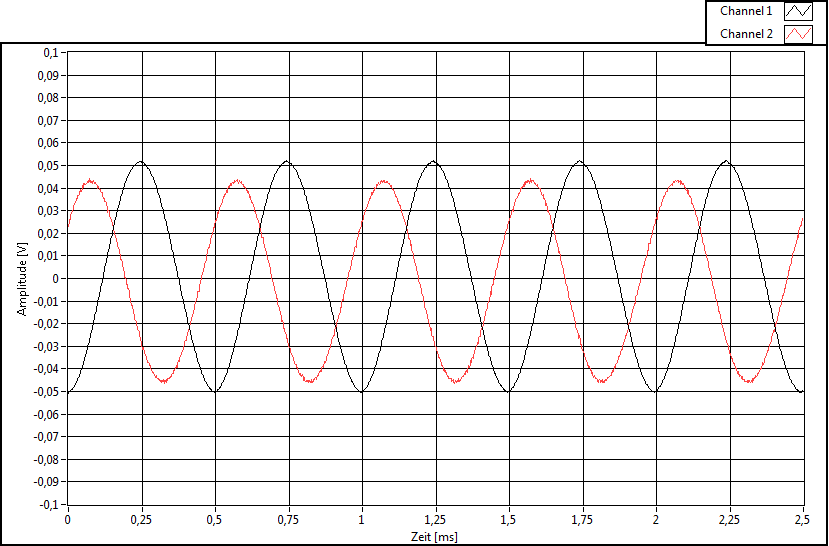
\includegraphics[width=\textwidth]{Sin50mV2kHz.png}
  \caption{50mV Amplitude}
  \label{fig:Sin50mV2kHz}
\end{figure}
\begin{figure}[H]
  \centering
    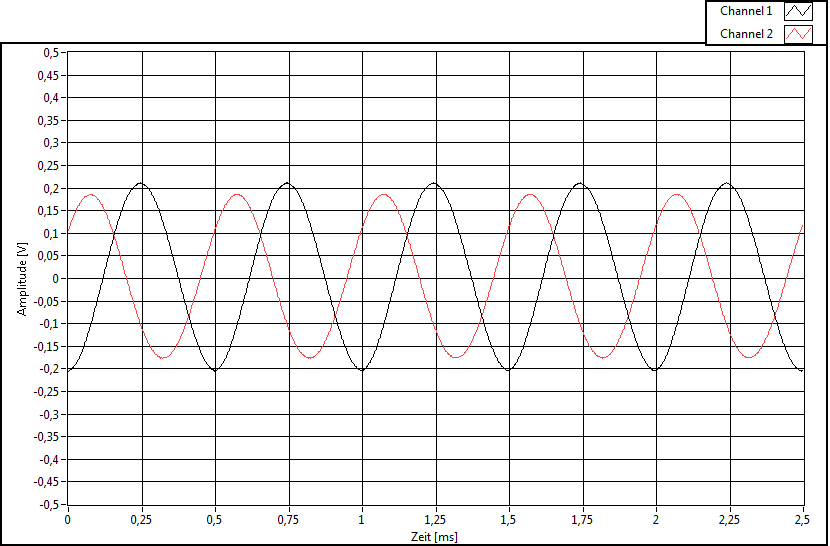
\includegraphics[width=\textwidth]{Sin200mV2kHz.png}
  \caption{200mV Amplitude}
  \label{fig:Sin200mV2kHz}
\end{figure}
\begin{figure}[H]
  \centering
    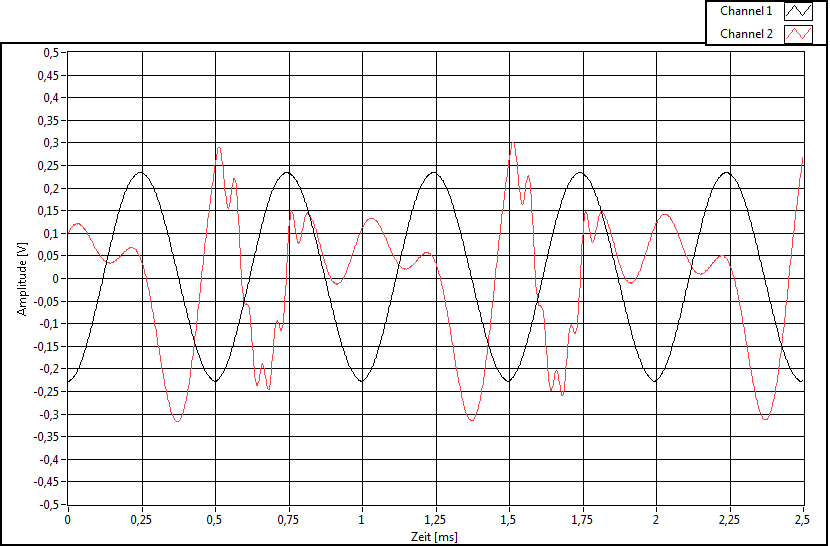
\includegraphics[width=\textwidth]{Sin230mV2kHz.png}
  \caption{230mV Amplitude}
  \label{fig:Sin230mV2kHz}
\end{figure}
Man sieht, dass das Ausgangssignal(rot) jeweils leicht gedämpft dem Eingangssignal entspricht außer bei 230mV Amplitude am Eingang. Der Erwartete Übersteuerungseffekt tritt also zwischen 200mV und 250mV auf. Dieses Ergebnis ist bei weitem besser als im Fall der Skalierung am Eingang.\\
Wir haben für die Fälle 50mV und 230mV die Spektren am Ausgang aufgenommen.\\
\begin{figure}[H]
  \centering
    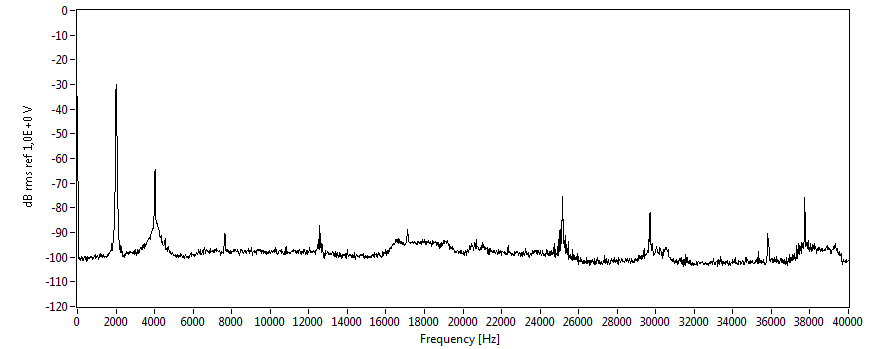
\includegraphics[width=\textwidth]{PowerSpektrumAusgang50mV2kHz.png}
  \caption{Spektrum am Ausgang 50mV}
  \label{fig:PowerSpektrumAusgang50mV2kHz}
\end{figure}
\begin{figure}[H]
  \centering
    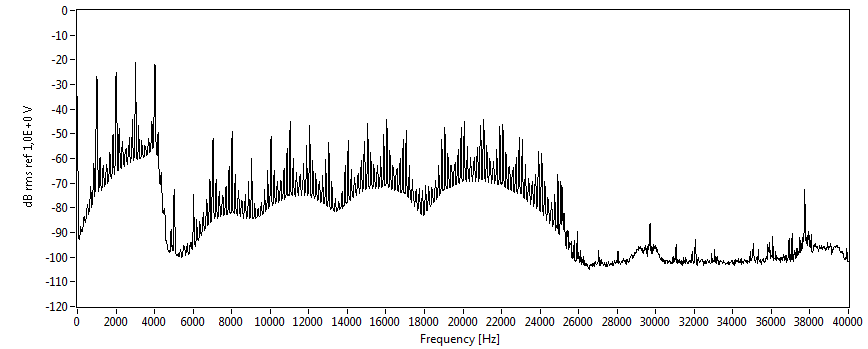
\includegraphics[width=\textwidth]{PowerSpektrumAusgang230mV2kHz.png}
  \caption{Spektrum am Ausgang 230mV}
  \label{fig:PowerSpektrumAusgang230mV2kHz}
\end{figure}
Bei dem Spektrum bei den 50mV ist das Ergebnis besser als bei der Skalierung am Eingang, so ist ein geringerer Rauschteppich sowie eine Stärkere Unterdrückung der höheren Harmonischen zu erkennen. Die erste Harmonische ist wie erwartet leicht gedämpft gut erkennbar. Das Spektrum der Variante mit 230mV ist wie erwartet nicht sehr eindeutig. Mit Fantasie erkennt man ein Tiefpassverhalten mit einer Grenzfrequenz um 4kHz, weitere Deutung lässt die Abbildung nicht zu.

\subsection{Optimierte Skalierung}
Der letzte Optimierungsschritt ist die Skalierung an jedem Teilfilter optimal passend zum Filter.
Dafür wurde folgendes Matlabfile erstellt.\\
\begin{adjustbox}{width=\textwidth,height=\textheight,keepaspectratio}
 \begin{lstlisting}[title=optimierung.m]
H1 = [-1 0 1 -0.9619429222893 1.847929303926];
H2 = [-1 0 1 -0.9633409060843 1.81768444585];
H3 = [-1 0 1 -0.9836465239584 1.819862361978];
H4 = [-1 0 1 -0.9850722601925 1.806715933748];

H=abs(freqz(H1(1:3),H1(4:5)));
g1=1/max(H);
H=g1*H;
H=H.*abs(freqz(H2(1:3),H2(4:5)));
g2=1/max(H);
H=g2*H;
H=H.*abs(freqz(H3(1:3),H3(4:5)));
g3=1/max(H);
H=g3*H;
H=H.*abs(freqz(H4(1:3),H4(4:5)));
g4=1/max(H);
H1n = (g1 .* H1(1:3) * 2^15)/2;
H2n = (g2 .* H2(1:3) * 2^15)/2;
H3n = (g3 .* H3(1:3) * 2^15)/2;
H4n = (g4 .* H4(1:3) * 2^15)/2;


\end{lstlisting}
\end{adjustbox}
Dieses Skript erstellt lediglich der Rechnung aus der Aufgabe entsprechend die einzelnen Skalierungsfaktoren und multipliziert diese mit den Filterkoeffizienten. Anschließend werden diese wieder in das handliche short Format gebracht.\\
Die neuen Filterkoeffizienten wurden daraufhin in das Programm gebracht.\\
\begin{adjustbox}{}
 \begin{lstlisting}[title=processdata.c]
const short coef[6*BIQUAD_STAGES] = {
	1,  427,    172,    427, -10390, 25748, //H4
	1, 3397,  -4336,   3397, -12529, 26454, //H3
	1, 9068, -14340,   9068, -14605, 27191, //H2
	1, 11981, -19529,  11981, -15896, 27808  //H1
};



int iDelayline[2*BIQUAD_STAGES+2];	// delayline for left and right channel samples

IIRstateStereo iirLR={coef,iDelayline,BIQUAD_STAGES};

void process_data()
{
	//!! Scale before filtering
	*(int*)(&sDAC1L) = iir_stereo(*(int*)(&sADC1L),&iirLR);
	//!! Scale after filtering

}
\end{lstlisting}
\end{adjustbox}
Man sieht, dass sich lediglich die Koeffizienten geändert haben und außerdem keinerlei Anpassung vorgenommen wurde.\\
Wir haben wie im Optimierungsfall zuvor die maximal mögliche Eingangsamplitude, die Fehlerfrei an den Ausgang gegeben wird ermittelt und visualisiert.
\begin{figure}[H]
  \centering
    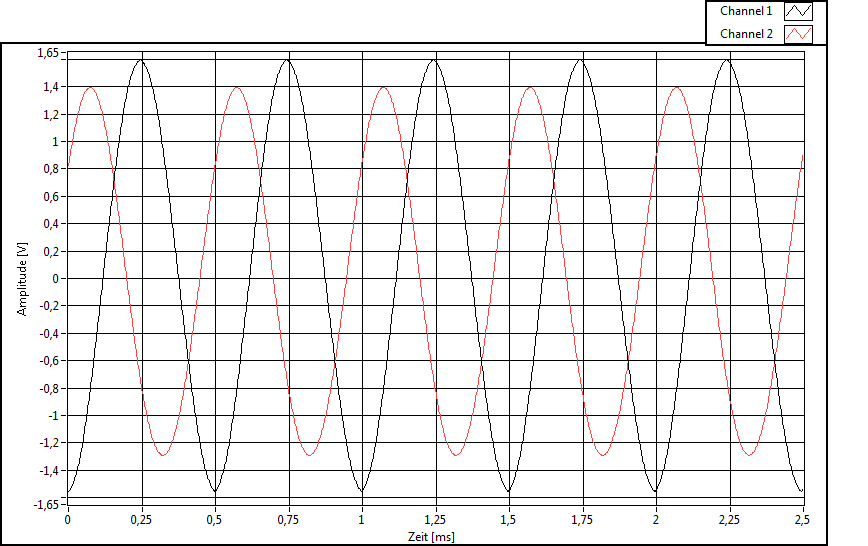
\includegraphics[width=\textwidth]{Sin1V61_2kHz.png}
  \caption{Sinus 1,61V}
  \label{fig:Sin1V61_2kHz}
\end{figure}
\begin{figure}[H]
  \centering
    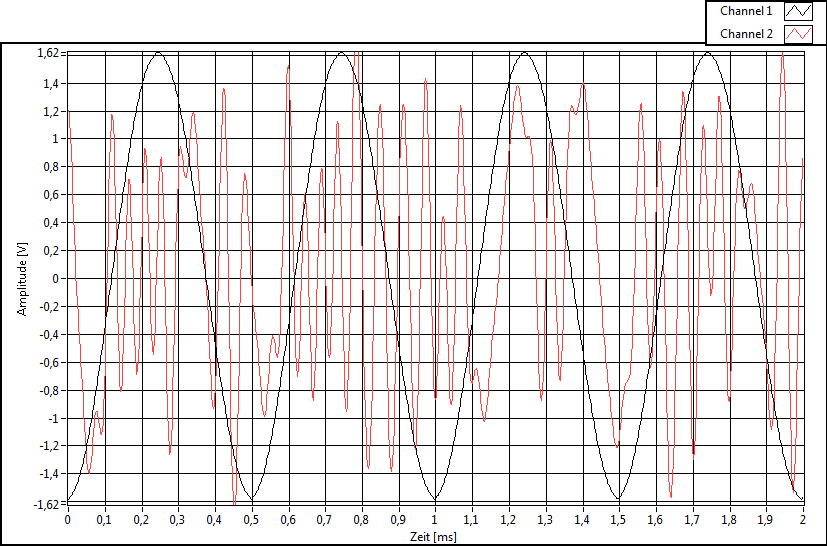
\includegraphics[width=\textwidth]{Sin1V62_2kHz.png}
  \caption{Sinus 1,62V}
  \label{fig:Sin1V62_2kHz}
\end{figure}
Es ist erkennbar, dass zwischen 1,61V und 1,62V Amplitude die Grenze liegt ab der der Fehler auftritt.
\begin{figure}[H]
  \centering
    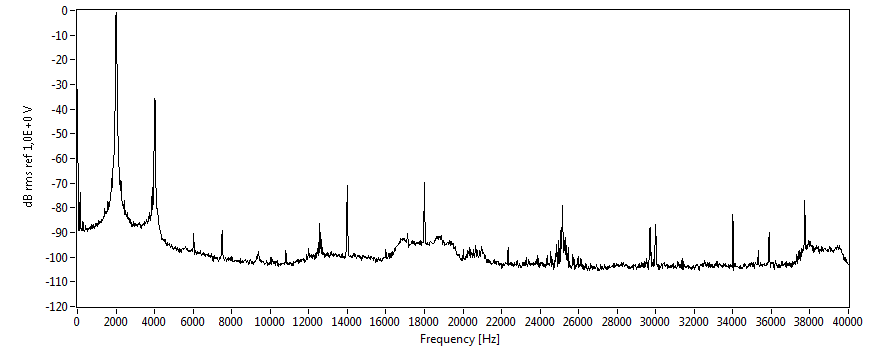
\includegraphics[width=\textwidth]{PowerSpektrumAusgang1V61_2kHz.png}
  \caption{Spektrum am Ausgang 1,61V}
  \label{fig:PowerSpektrumAusgang1V61_2kHz}
\end{figure}
\begin{figure}[H]
  \centering
    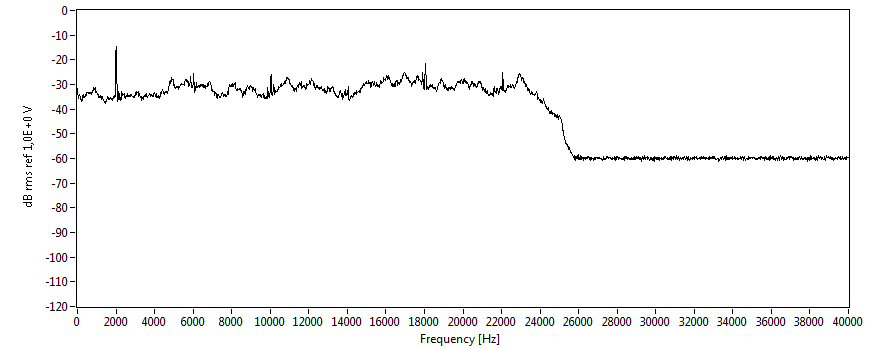
\includegraphics[width=\textwidth]{PowerSpektrumAusgang1V62_2kHz.png}
  \caption{Spektrum am Ausgang 1,62V}
  \label{fig:PowerSpektrumAusgang1V62_2kHz}
\end{figure}
Bei der Version mit 1,61V Amplitude ist der Peak bei 2kHz eindeutig zu erkennen, genau wie die erste Harmonische bei 4kHz, wie erwartet leicht gedämpft. Bei 1,62V Amplitude ist wie erwartet kein befriedigendes Ergebnis vorhanden, was bestätigt, dass die Grenzamplitude ab der das Übersteuern zwischen 1,61V und 1,62V liegt.\\ 
Als Resultat lässt sich festhalten, dass die letzte Variante der optimierten Anpassung zum Besten Ergebnis führt, da hier die höchste Amplitude ohne Fehler auftritt. Diese Implementierung hat zwar den höchsten Implementierungsaufwand, aber keine Performancenachteile, da die Filterkoeffizienten hart gecodet wurden.
